\documentclass{standalone}
\usepackage{tikz, ifthen}
\usepackage{amsmath}

\begin{document}

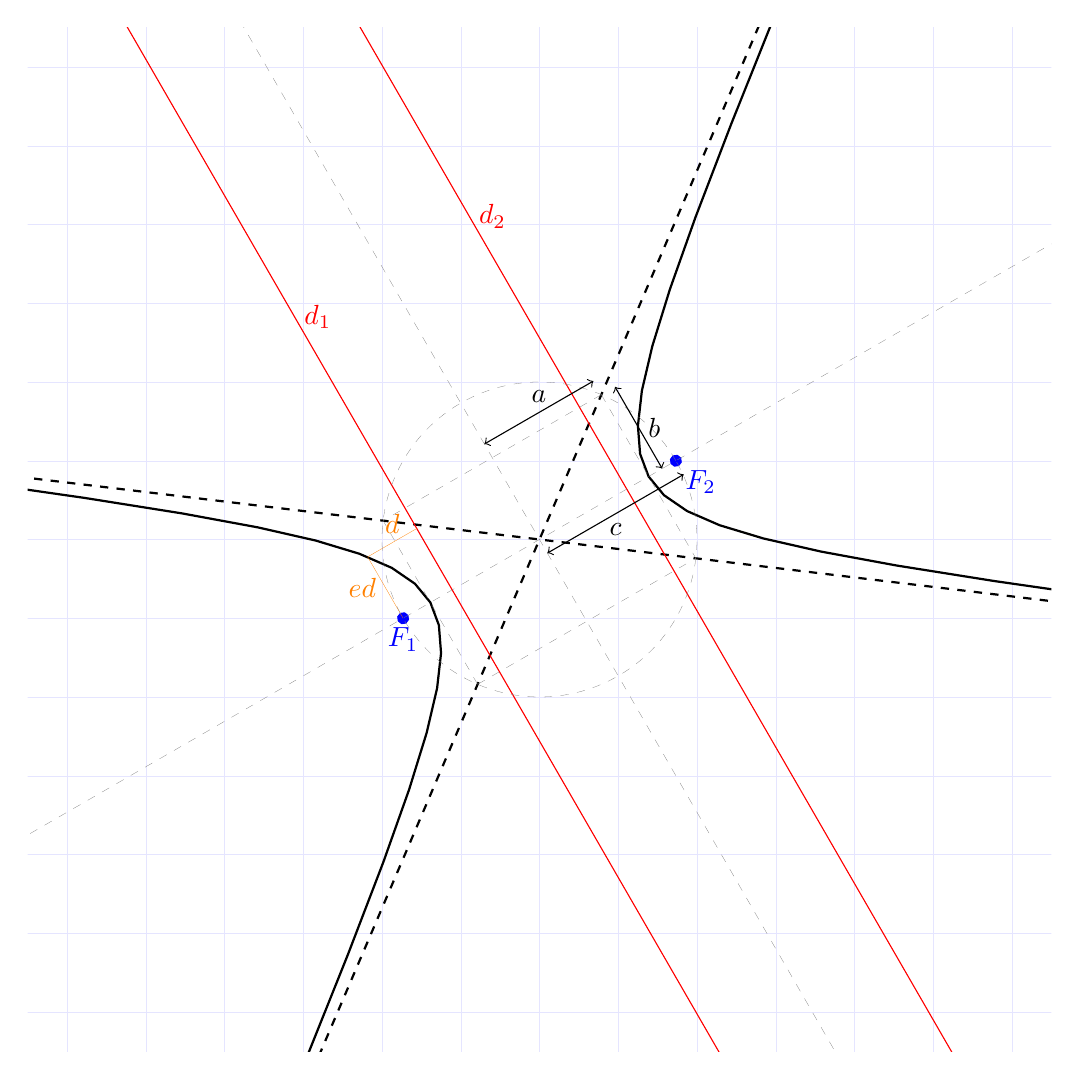
\begin{tikzpicture}
    
    % Center of the circle
    \def\xmin{-6}
    \def\xmax{6}
    \def\ymin{-6}
    \def\ymax{6}
    \def\dx{.5}
    \def\dy{.5}
    \def\xminb{\xmin-\dx}
    \def\xmaxb{\xmax+\dx}
    \def\yminb{\ymin-\dy}
    \def\ymaxb{\ymax+\dy}
    \def\xa{-2}     % x focus A 
    \def\ya{ 0}     % y focus A
    \def\xb{ 2}     % x focus B
    \def\yb{ 0}     % y focus B
    \def\xpmin{-6}
    \def\xpmax{ 6}
    \def\ypmin{-5.5}
    \def\ypmax{ 5.5}
    \def\a{1.6};
    \coordinate (fa) at (\xa, \ya);
    \coordinate (fb) at (\xb, \yb);
    \def\c{sqrt((\xb-\xa)*(\xb-\xa)+(\ya-\yb)*(\ya-\yb))/2};
    \def\xc{0.5*(\xa+\xb)};
    \def\yc{0.5*(\ya+\yb)};
    \coordinate (center) at ({\xc}, {\yc});
    \def\b{sqrt(\c*\c-\a*\a)};
    \def\e{(\c/\a)}
    \def\ed{\c*(\e*\e-1)/\e}
    \def\d{\ed/\e}
%   \def\alpha{{atan2(\yb-\ya,\xb-\xa)}};
    \def\alpha{30}

    \clip (\xminb, \yminb) rectangle (\xmaxb, \ymaxb);

    % Draw grid
    \draw[step=1., blue!10, ultra thin] (\xmin-2, \ymin-2) grid (\xmax+2, \ymax+2); % Visible grid with lighter color

%   % Axes, x
%   \draw[->, thick, blue] (\xmin, 0) -- (\xmax, 0) node[below right] {$x$};
%   \draw[    thick, blue] (\xmin-2, 0) -- (\xmax+2, 0);
%   \draw[->, thick, blue] (0, \ymin) -- (0, \ymax) node[right] {$y$};
%   \draw[    thick, blue] (0, \ymin-2) -- (0, \ymax+2);
%   % Axis ticks
%   \foreach \x in {\xmin,..., \xmax}{
%       \ifthenelse{ \x = 0 }{}{\draw[blue] (\x, -0.1) -- (\x, +0.1) node[below=8pt, left=0pt] {\small $\x$};}
%   }
%   \foreach \y in {\ymin,..., \ymax}{
%       \ifthenelse{ \y = 0 }{}{\draw[blue] (-0.1, \y) -- (0.1, \y) node[left=4pt] {\small $\y$};}
%   }
    
    % Hyperbola branch 1
    \draw[thick, black, rotate=\alpha] plot[parametric, domain=-3:3] ({ \xc+\a*cosh(\x)}, {\yc+\b*sinh(\x)}); % Branch 1
    \draw[thick, black, rotate=\alpha] plot[parametric, domain=-3:3] ({-\xc-\a*cosh(\x)}, {\yc+\b*sinh(\x)}); % Branch 2
    % Asymptotes
    \draw[thick, dashed, rotate=\alpha] ({-10*\a},{-10*\b}) -- ({ 10*\a}, {10*\b});
    \draw[thick, dashed, rotate=\alpha] ({ 10*\a},{-10*\b}) -- ({-10*\a}, {10*\b});
    % Foci
    \filldraw[blue, rotate=\alpha] ({-\c},0) circle (2pt) node[below      ] {$F_1$};
    \filldraw[blue, rotate=\alpha] ({ \c},0) circle (2pt) node[below right] {$F_2$};
    % Directrices
    \filldraw[red, rotate=\alpha] ({-\d+\c},{-10}) -- ({-\d+\c}, {10});
    \filldraw[red, rotate=\alpha] ({ \d-\c},{-10}) -- ({ \d-\c}, {10});
    \filldraw[red, rotate=\alpha] ({-\c+\d},4) circle (0) node[right] {$d_1$};
    \filldraw[red, rotate=\alpha] ({ \c-\d},4) circle (0) node[right] {$d_2$};
    % Semi-latus rectum
    \draw[ultra thin, orange, rotate=\alpha] ({-\c},0      ) -- ({-\c   },{\ed}) node[midway, left ] {$ed$};
    \draw[ultra thin, orange, rotate=\alpha] ({-\c},{(\ed)}) -- ({-\c+\d},{\ed}) node[midway, above] {$d$};

    % Construction lines
    \draw[ultra thin, black!50, dashed, rotate=\alpha] (0,-10) -- (0,10);
    \draw[ultra thin, black!50, dashed, rotate=\alpha] (-10,0) -- (10,0);
    \draw[ultra thin, black!50, dashed, rotate=\alpha] (0,0) circle (\c);
    % Rectangle
    \draw[ultra thin, black!50, dashed, rotate=\alpha] ({-\a},{-\b}) -- ({ \a},{-\b});
    \draw[ultra thin, black!50, dashed, rotate=\alpha] ({-\a},{-\b}) -- ({-\a},{ \b});
    \draw[ultra thin, black!50, dashed, rotate=\alpha] ({ \a},{ \b}) -- ({ \a},{-\b});
    \draw[ultra thin, black!50, dashed, rotate=\alpha] ({ \a},{ \b}) -- ({-\a},{ \b});

    % Measurements
    \draw[<->, black, rotate=\alpha] (0,{  -0.2})     -- ({\c},{  -0.2})      node [midway, below] {$c$};
    \draw[<->, black, rotate=\alpha] (0,{\b+0.2})     -- ({\a},{\b+0.2})      node [midway, above] {$a$};
    \draw[<->, black, rotate=\alpha] ({  \a+0.2},{0}) -- ({     \a+0.2},{\b}) node [midway, right] {$b$};

%   \draw[dashed] (-\a,-\b) -- ( \a,-\b);
%   \draw[dashed] (-\a,-\b) -- (-\a, \b);
%   \draw[dashed] ( \a, \b) -- ( \a,-\b);
%   \draw[dashed] ( \a, \b) -- (-\a,-\b);

%     % Axes, x'
%     \draw[->, thick, red, rotate=30] (\xmin, \yo) -- (\xmax, \yo) node[right] {$x'$};
%     \draw[->, thick, red, rotate=30] (\xo, \ymin) -- (\xo, \ymax) node[right] {$y'$};
%     \draw[    thick, red, rotate=30] (\xmin-2, 0) -- (\xmax+2, 0);
%     \draw[    thick, red, rotate=30] (0, \ymin-2) -- (0, \ymax+2);
%     % Axis thick
%     \foreach \x in {\xmin,..., \xmax}{
%         \ifthenelse{ \x = 0 }{}{\draw[red, rotate=30] (\x+\xo, \yo-0.1) -- (\x+\xo, \yo+0.1) node[below=8pt, left=0pt] {\small $\x$};}
%     }
%     \foreach \y in {\ymin,...,\ymax}{
%         \ifthenelse{ \y = 0 }{}{\draw[red, rotate=30] (\xo-0.1, \yo+\y) -- (\xo+0.1, \yo+\y) node[left=4pt] {\small $\y$};}
%     }
%     % Origin
%     \filldraw[blue] (0,0) circle (2pt) node[below=7pt, right=-13pt] {$O$};
%     \filldraw[red] (\xo,\yo) circle (2pt) node[below=7pt, right=-3pt] {$\equiv O'$};

%   \filldraw[blue]  (3,5) circle (1pt) node[below right] {$\equiv (3,5)$};
%   \filldraw[red]   (3,5) circle (1pt) node[below=20pt, right] {$\equiv (1,3.5)$};
%   \filldraw[black] (3,5) circle (2pt) node[below left] {$A$};

%   \filldraw[blue]  (-4,3) circle (1pt) node[below right] {$\equiv (-4,3)$};
%   \filldraw[red]   (-4,3) circle (1pt) node[below=20pt, right] {$\equiv (-6,1.5)$};
%   \filldraw[black] (-4,3) circle (2pt) node[below left] {$B$};

%   \filldraw[blue]  (1,-4) circle (1pt) node[right=12pt] {$\equiv (1,-4)$};
%   \filldraw[red]   (1,-4) circle (1pt) node[right=55pt] {$\equiv (-1,-5.5)$};
%   \filldraw[black] (1,-4) circle (2pt) node[right] {$C$};

%   % Foci
%   \filldraw[blue] (\xa, \ya) circle (2pt) node[above right] {$0$};
%   \filldraw[blue] (\xb, \yb) circle (2pt) node[above right] {$2$};
    
\end{tikzpicture}

\end{document}
